% Options for packages loaded elsewhere
\PassOptionsToPackage{unicode}{hyperref}
\PassOptionsToPackage{hyphens}{url}
%
\documentclass[
]{article}
\usepackage{amsmath,amssymb}
\usepackage{lmodern}
\usepackage{iftex}
\ifPDFTeX
  \usepackage[T1]{fontenc}
  \usepackage[utf8]{inputenc}
  \usepackage{textcomp} % provide euro and other symbols
\else % if luatex or xetex
  \usepackage{unicode-math}
  \defaultfontfeatures{Scale=MatchLowercase}
  \defaultfontfeatures[\rmfamily]{Ligatures=TeX,Scale=1}
\fi
% Use upquote if available, for straight quotes in verbatim environments
\IfFileExists{upquote.sty}{\usepackage{upquote}}{}
\IfFileExists{microtype.sty}{% use microtype if available
  \usepackage[]{microtype}
  \UseMicrotypeSet[protrusion]{basicmath} % disable protrusion for tt fonts
}{}
\makeatletter
\@ifundefined{KOMAClassName}{% if non-KOMA class
  \IfFileExists{parskip.sty}{%
    \usepackage{parskip}
  }{% else
    \setlength{\parindent}{0pt}
    \setlength{\parskip}{6pt plus 2pt minus 1pt}}
}{% if KOMA class
  \KOMAoptions{parskip=half}}
\makeatother
\usepackage{xcolor}
\usepackage[margin=1in]{geometry}
\usepackage{color}
\usepackage{fancyvrb}
\newcommand{\VerbBar}{|}
\newcommand{\VERB}{\Verb[commandchars=\\\{\}]}
\DefineVerbatimEnvironment{Highlighting}{Verbatim}{commandchars=\\\{\}}
% Add ',fontsize=\small' for more characters per line
\usepackage{framed}
\definecolor{shadecolor}{RGB}{248,248,248}
\newenvironment{Shaded}{\begin{snugshade}}{\end{snugshade}}
\newcommand{\AlertTok}[1]{\textcolor[rgb]{0.94,0.16,0.16}{#1}}
\newcommand{\AnnotationTok}[1]{\textcolor[rgb]{0.56,0.35,0.01}{\textbf{\textit{#1}}}}
\newcommand{\AttributeTok}[1]{\textcolor[rgb]{0.77,0.63,0.00}{#1}}
\newcommand{\BaseNTok}[1]{\textcolor[rgb]{0.00,0.00,0.81}{#1}}
\newcommand{\BuiltInTok}[1]{#1}
\newcommand{\CharTok}[1]{\textcolor[rgb]{0.31,0.60,0.02}{#1}}
\newcommand{\CommentTok}[1]{\textcolor[rgb]{0.56,0.35,0.01}{\textit{#1}}}
\newcommand{\CommentVarTok}[1]{\textcolor[rgb]{0.56,0.35,0.01}{\textbf{\textit{#1}}}}
\newcommand{\ConstantTok}[1]{\textcolor[rgb]{0.00,0.00,0.00}{#1}}
\newcommand{\ControlFlowTok}[1]{\textcolor[rgb]{0.13,0.29,0.53}{\textbf{#1}}}
\newcommand{\DataTypeTok}[1]{\textcolor[rgb]{0.13,0.29,0.53}{#1}}
\newcommand{\DecValTok}[1]{\textcolor[rgb]{0.00,0.00,0.81}{#1}}
\newcommand{\DocumentationTok}[1]{\textcolor[rgb]{0.56,0.35,0.01}{\textbf{\textit{#1}}}}
\newcommand{\ErrorTok}[1]{\textcolor[rgb]{0.64,0.00,0.00}{\textbf{#1}}}
\newcommand{\ExtensionTok}[1]{#1}
\newcommand{\FloatTok}[1]{\textcolor[rgb]{0.00,0.00,0.81}{#1}}
\newcommand{\FunctionTok}[1]{\textcolor[rgb]{0.00,0.00,0.00}{#1}}
\newcommand{\ImportTok}[1]{#1}
\newcommand{\InformationTok}[1]{\textcolor[rgb]{0.56,0.35,0.01}{\textbf{\textit{#1}}}}
\newcommand{\KeywordTok}[1]{\textcolor[rgb]{0.13,0.29,0.53}{\textbf{#1}}}
\newcommand{\NormalTok}[1]{#1}
\newcommand{\OperatorTok}[1]{\textcolor[rgb]{0.81,0.36,0.00}{\textbf{#1}}}
\newcommand{\OtherTok}[1]{\textcolor[rgb]{0.56,0.35,0.01}{#1}}
\newcommand{\PreprocessorTok}[1]{\textcolor[rgb]{0.56,0.35,0.01}{\textit{#1}}}
\newcommand{\RegionMarkerTok}[1]{#1}
\newcommand{\SpecialCharTok}[1]{\textcolor[rgb]{0.00,0.00,0.00}{#1}}
\newcommand{\SpecialStringTok}[1]{\textcolor[rgb]{0.31,0.60,0.02}{#1}}
\newcommand{\StringTok}[1]{\textcolor[rgb]{0.31,0.60,0.02}{#1}}
\newcommand{\VariableTok}[1]{\textcolor[rgb]{0.00,0.00,0.00}{#1}}
\newcommand{\VerbatimStringTok}[1]{\textcolor[rgb]{0.31,0.60,0.02}{#1}}
\newcommand{\WarningTok}[1]{\textcolor[rgb]{0.56,0.35,0.01}{\textbf{\textit{#1}}}}
\usepackage{graphicx}
\makeatletter
\def\maxwidth{\ifdim\Gin@nat@width>\linewidth\linewidth\else\Gin@nat@width\fi}
\def\maxheight{\ifdim\Gin@nat@height>\textheight\textheight\else\Gin@nat@height\fi}
\makeatother
% Scale images if necessary, so that they will not overflow the page
% margins by default, and it is still possible to overwrite the defaults
% using explicit options in \includegraphics[width, height, ...]{}
\setkeys{Gin}{width=\maxwidth,height=\maxheight,keepaspectratio}
% Set default figure placement to htbp
\makeatletter
\def\fps@figure{htbp}
\makeatother
\setlength{\emergencystretch}{3em} % prevent overfull lines
\providecommand{\tightlist}{%
  \setlength{\itemsep}{0pt}\setlength{\parskip}{0pt}}
\setcounter{secnumdepth}{-\maxdimen} % remove section numbering
\ifLuaTeX
  \usepackage{selnolig}  % disable illegal ligatures
\fi
\IfFileExists{bookmark.sty}{\usepackage{bookmark}}{\usepackage{hyperref}}
\IfFileExists{xurl.sty}{\usepackage{xurl}}{} % add URL line breaks if available
\urlstyle{same} % disable monospaced font for URLs
\hypersetup{
  pdftitle={Wk5 Quiz Notes},
  pdfauthor={D. ODay},
  hidelinks,
  pdfcreator={LaTeX via pandoc}}

\title{Wk5 Quiz Notes}
\author{D. ODay}
\date{2022-07-13}

\begin{document}
\maketitle

\begin{Shaded}
\begin{Highlighting}[]
\FunctionTok{require}\NormalTok{(lolcat)}
\end{Highlighting}
\end{Shaded}

\begin{verbatim}
## Loading required package: lolcat
\end{verbatim}

\begin{verbatim}
## lolcat 2.0.0
\end{verbatim}

\begin{Shaded}
\begin{Highlighting}[]
\FunctionTok{require}\NormalTok{(dplyr)}
\end{Highlighting}
\end{Shaded}

\begin{verbatim}
## Loading required package: dplyr
\end{verbatim}

\begin{verbatim}
## 
## Attaching package: 'dplyr'
\end{verbatim}

\begin{verbatim}
## The following objects are masked from 'package:stats':
## 
##     filter, lag
\end{verbatim}

\begin{verbatim}
## The following objects are masked from 'package:base':
## 
##     intersect, setdiff, setequal, union
\end{verbatim}

\hypertarget{question-1-which-hypothesis-is-generally-related-to-the-research-question}{%
\section{Question 1: Which hypothesis is generally related to the
research
question?}\label{question-1-which-hypothesis-is-generally-related-to-the-research-question}}

-should be alternative

\hypertarget{question-2-test-statistics-are}{%
\section{Question 2: Test statistics
are:}\label{question-2-test-statistics-are}}

\begin{itemize}
\tightlist
\item
  standardized statistics that have defined probabilities distributions
\end{itemize}

\hypertarget{question-3-true-or-false-a-researcher-is-more-likely-to-make-a-type-i-error-with-a-directional-one-tailed-test-than-with-a-non-directional-two-tailed-test.}{%
\section{Question 3: True or False: A researcher is more likely to make
a Type I error with a directional (one-tailed) test than with a
non-directional (two-tailed)
test.}\label{question-3-true-or-false-a-researcher-is-more-likely-to-make-a-type-i-error-with-a-directional-one-tailed-test-than-with-a-non-directional-two-tailed-test.}}

\begin{itemize}
\tightlist
\item
  True
\end{itemize}

\hypertarget{question-4-true-or-false-power-is-the-ability-to-detect-a-true-difference-when-it-exists.}{%
\section{Question 4: True or False: Power is the ability to detect a
true difference when it
exists.}\label{question-4-true-or-false-power-is-the-ability-to-detect-a-true-difference-when-it-exists.}}

\begin{itemize}
\tightlist
\item
  true
\end{itemize}

\hypertarget{question-5-a-new-drug-therapy-is-being-tested-for-efficacy-as-compared-to-a-placebo.the-results-of-the-study-say-that-a-statistically-significant-difference-exists-but-in-reality-there-is-no-difference-from-the-placebo.-this-is-an-example-of-______________.}{%
\section{Question 5: A new drug therapy is being tested for efficacy as
compared to a placebo.The results of the study say that a statistically
significant difference exists, but in reality, there is no difference
from the placebo. This is an example of
\_\_\_\_\_\_\_\_\_\_\_\_\_\_.}\label{question-5-a-new-drug-therapy-is-being-tested-for-efficacy-as-compared-to-a-placebo.the-results-of-the-study-say-that-a-statistically-significant-difference-exists-but-in-reality-there-is-no-difference-from-the-placebo.-this-is-an-example-of-______________.}}

\begin{itemize}
\tightlist
\item
  A Type I Error
\end{itemize}

\hypertarget{question-6-when-h0-is-false-and-we-accept-h0-which-of-the-following-describe-what-has-occurred-choose-all-that-are-correct}{%
\section{Question 6: When H0 is False and we Accept H0 which of the
following describe what has occurred? (choose all that are
correct):}\label{question-6-when-h0-is-false-and-we-accept-h0-which-of-the-following-describe-what-has-occurred-choose-all-that-are-correct}}

\begin{itemize}
\tightlist
\item
  Type II Error
\item
  Probability = \(\beta\)
\end{itemize}

\#Q7:If management has initially identified the requirements of a
hardness test to be ⍺ = 0.01, Δ𝛍 = 1, n = 20 and 𝛔 was estimated to be
2.0, what would the power be for to detect a change in the Mean? Record
your answer to 4 places after the decimal point (e.g.~X.XXXX).

\begin{Shaded}
\begin{Highlighting}[]
\FunctionTok{power.mean.t.onesample}\NormalTok{(}\AttributeTok{sample.size =} \DecValTok{20}
\NormalTok{                       ,}\AttributeTok{effect.size =} \DecValTok{1}
\NormalTok{                       ,}\AttributeTok{variance.est =} \DecValTok{2}\SpecialCharTok{\^{}}\DecValTok{2}
\NormalTok{                       ,}\AttributeTok{alpha =} \FloatTok{0.01}
\NormalTok{                       ,}\AttributeTok{alternative =}\StringTok{"two.sided"}\NormalTok{)}
\end{Highlighting}
\end{Shaded}

\begin{verbatim}
##   test       type alternative sample.size actual df effect.size variance alpha
## 1    t one.sample   two.sided          20     20 19           1        4  0.01
##   conf.level      beta     power
## 1       0.99 0.7026557 0.2973443
\end{verbatim}

\begin{Shaded}
\begin{Highlighting}[]
\CommentTok{\#0.2973}
\end{Highlighting}
\end{Shaded}

\#Q8: If management has initially identified the requirements of a
hardness test to be ⍺ = 0.01, β = 0.05, Δ𝛍 = 1, and 𝛔 was estimated to
be 2.0, what would be the minimum sample size needed to to detect a
change in the Mean? Record your answer as an integer (e.g.~XX).

\begin{Shaded}
\begin{Highlighting}[]
\FunctionTok{sample.size.mean.t.onesample}\NormalTok{(}\AttributeTok{beta =} \FloatTok{0.05}
\NormalTok{                       ,}\AttributeTok{effect.size =} \DecValTok{1}
\NormalTok{                       ,}\AttributeTok{variance.est =} \DecValTok{2}\SpecialCharTok{\^{}}\DecValTok{2}
\NormalTok{                       ,}\AttributeTok{alpha =} \FloatTok{0.01}
\NormalTok{                       ,}\AttributeTok{alternative =}\StringTok{"two.sided"}\NormalTok{)}
\end{Highlighting}
\end{Shaded}

\begin{verbatim}
##   test       type alternative sample.size actual df effect.size variance alpha
## 1    t one.sample   two.sided          75     75 74           1        4  0.01
##   conf.level beta     power
## 1       0.99 0.05 0.9511756
\end{verbatim}

\begin{Shaded}
\begin{Highlighting}[]
\CommentTok{\#75}
\end{Highlighting}
\end{Shaded}

\#Q9: In a two-tailed situation, there are two different effects and
sample sizes that need to be computed when doing the computations based
on variances. - True

\#Q10: When a linking procedure (matching, blocking, pairing) is used to
create dependent samples, those samples will be: - Dependent by design
(but still independent by nature)

\#A company is investigating two types of hearing protection devices to
decrease the effective noise level experienced by its employees, either
earmuffs or foam earplugs. The earmuffs are considerably more expensive,
and the president wants to know at the 0.05 level of significance
whether this expenditure has resulted in a change in the mean level of
effective noise level. The sample results are shown below

\begin{itemize}
\tightlist
\item
  Earmuffs

  \begin{itemize}
  \tightlist
  \item
    mean = 72
  \item
    n = 12
  \item
    sd = 15 -Foam Earplugs
  \item
    mean = 64
  \item
    n = 15
  \item
    sd = 19
  \end{itemize}
\end{itemize}

\#Q11: What is the value of the test statistic? Record your answer to 4
places \# after the decimal point (e.g.~X.XXXX) Also, Q12, 13

\begin{Shaded}
\begin{Highlighting}[]
\CommentTok{\#0.2451}
\FunctionTok{t.test.twosample.independent.simple}\NormalTok{(}\AttributeTok{sample.mean.g1 =} \DecValTok{72}\NormalTok{,}
                                    \AttributeTok{sample.variance.g1 =} \DecValTok{15} \SpecialCharTok{*} \DecValTok{15}\NormalTok{, }
                                    \AttributeTok{sample.size.g1 =} \DecValTok{12}\NormalTok{, }
                                    \AttributeTok{sample.mean.g2 =} \DecValTok{64}\NormalTok{, }
                                    \AttributeTok{sample.variance.g2 =} \DecValTok{19} \SpecialCharTok{*} \DecValTok{19}\NormalTok{, }
                                    \AttributeTok{sample.size.g2 =} \DecValTok{15}\NormalTok{, }
                                    \AttributeTok{conf.level =} \FloatTok{0.95}\NormalTok{)}
\end{Highlighting}
\end{Shaded}

\begin{verbatim}
## 
##  Two-Sample t Test For Means (Equal Variances)
## 
## data:  input sample means and variances
## t statistic = 1.1903, null hypothesis difference = 0, p-value = 0.2451
## alternative hypothesis: true difference of means is not equal to 0
## 95 percent confidence interval:
##  -5.842489 21.842489
## sample estimates:
##                diff              se.est                  df             g1.mean 
##           8.0000000           6.7211606          25.0000000          72.0000000 
##     g1.mean.lowerci     g1.mean.upperci      g1.sample.size              g1.var 
##          62.4694547          81.5305453          12.0000000         225.0000000 
##      g1.var.lowerci      g1.var.upperci               g1.sd       g1.sd.lowerci 
##         112.9103302         648.6276967          15.0000000          10.6259273 
##       g1.sd.upperci             g2.mean     g2.mean.lowerci     g2.mean.upperci 
##          25.4681703          64.0000000          53.4781507          74.5218493 
##      g2.sample.size              g2.var      g2.var.lowerci      g2.var.upperci 
##          15.0000000         361.0000000         193.4993703         897.8941074 
##               g2.sd       g2.sd.lowerci       g2.sd.upperci var.test.conf.level 
##          19.0000000          13.9104051          29.9648812           0.9500000 
##          var.test.F      var.test.df.g1      var.test.df.g2          var.test.p 
##           0.6232687          11.0000000          14.0000000           0.4358964
\end{verbatim}

\begin{Shaded}
\begin{Highlighting}[]
\NormalTok{ToolLife }\OtherTok{\textless{}{-}} \FunctionTok{read.delim}\NormalTok{(}\StringTok{"\textasciitilde{}/Documents/GitHub/school\_cu/school\_cu/methods for quality improvement/DTSA5704\_DescribingData/data/ToolLife.dat"}\NormalTok{)}
\end{Highlighting}
\end{Shaded}

\begin{Shaded}
\begin{Highlighting}[]
\NormalTok{ToolLife }\SpecialCharTok{\%\textgreater{}\%} \FunctionTok{group\_by}\NormalTok{(vendor) }\SpecialCharTok{\%\textgreater{}\%} \FunctionTok{summarise}\NormalTok{(}
  \AttributeTok{mean1 =} \FunctionTok{mean}\NormalTok{(life),}
  \AttributeTok{variance =} \FunctionTok{var}\NormalTok{(life)}
\NormalTok{)}
\end{Highlighting}
\end{Shaded}

\begin{verbatim}
## # A tibble: 2 x 3
##   vendor mean1 variance
##    <int> <dbl>    <dbl>
## 1      1  52.4     78.2
## 2      2  38.0    254.
\end{verbatim}

\#Q14,15,16: Question 14 One of the many consumable supplies that a
company's Purchasing Department is responsible for obtaining is cutter
inserts for their lathe operations. The purchasing manager previously
elected to buy an equal volume of cutters from two suppliers. The lathe
operators, through time, had been reporting to their department
supervisor that there was a difference between the two vendors' cutter
inserts in terms of cutting life. The supervisor decided to
statistically test whether there was really a difference in the average
cutting life between the two vendors' inserts. She requested that her
operators use the inserts fromthe two suppliers in a random fashion
across the parts being machined and to record the total cutting time
(life) for each of the inserts.

When sufficient data were compiled, the supervisor organized the
obtained values as shown below, and saved them in a file named
TOOLLIFE.DAT. The insert life was recorded in minutes. Assist the
supervisor in conducting the appropriate analysis required to answer the
research question

-Which Vendor has the higher mean? - Vendor 1 - Which Vendor has the
higher variance? - Vendor 2 - Means

\#Q17, 18, 19

Question 18 A steel bar straightening machine has been in use for 15
years. When the machine was purchased (prior to the implementation of
quality improvement policies), it was assumed that it would perform as
advertised. That is, it would significantly improve the straightness of
the product. The process engineer had just recently attended a stats
course in R. They became anxious to statistically test whether the
straightening operation was changing the process mean for bar
straightness.

20 bars were randomly selected from a production lot and identified in a
serial fashion. It was then arranged to have an inspector measure the
straightness of each bar. Subsequently, the bars were put through the
straightening operation. Each of the bars was remeasured for
straightness after the operation by the same inspector.

Because the measurements were repeated on the same parts and the data
were paired according to the bar identification, we have data that are
dependent by nature. The first column contains the straightness values
measured prior to the operation and the second column contains the
values measured after the operation. The values in each row represent
the same specimen, in this case, a bar. A flat bar has a value of zero,
a non-flat bar has values above zero. The data file is named
Straight.dat.

Has the straightening operation significantly changed the process mean?
Has the straightness of the population of bars been improved? Assume an
⍺ of 0.010.

\begin{Shaded}
\begin{Highlighting}[]
\NormalTok{Straight }\OtherTok{\textless{}{-}} \FunctionTok{read.delim}\NormalTok{(}\StringTok{"\textasciitilde{}/Documents/GitHub/school\_cu/school\_cu/methods for quality improvement/DTSA5704\_DescribingData/data/Straight.dat"}\NormalTok{)}
\end{Highlighting}
\end{Shaded}

\begin{itemize}
\tightlist
\item
  What is the source of the dependency? -Repeated Measures
\end{itemize}

\begin{Shaded}
\begin{Highlighting}[]
\NormalTok{Straight}\SpecialCharTok{$}\NormalTok{Diff }\OtherTok{=}\NormalTok{ Straight}\SpecialCharTok{$}\NormalTok{before }\SpecialCharTok{{-}}\NormalTok{ Straight}\SpecialCharTok{$}\NormalTok{after}
\FunctionTok{t.test.twosample.dependent}\NormalTok{(}\AttributeTok{x1 =}\NormalTok{ Straight}\SpecialCharTok{$}\NormalTok{before,}\AttributeTok{x2 =}\NormalTok{ Straight}\SpecialCharTok{$}\NormalTok{after)}
\end{Highlighting}
\end{Shaded}

\begin{verbatim}
## 
##  Dependent Samples t Test for Means (D-bar method)
## 
## data:  sample mean, sample size, and estimated variance
## t statistic = -0.90874, null hypothesis mean = 0, p-value = 0.3749
## alternative hypothesis: true mean is not equal to 0
## 95 percent confidence interval:
##  -0.003798686  0.001498686
## sample estimates:
##   sample.mean        se.est            df   var.lowerci           var 
## -1.150000e-03  1.265483e-03  1.900000e+01  1.852380e-05  3.202895e-05 
##   var.upperci    sd.lowerci            sd    sd.upperci         power 
##  6.832638e-05  4.303929e-03  5.659412e-03  8.265977e-03  1.364392e-01
\end{verbatim}

\#Q20\_21\_22

A plant superintendent has been assigned the task of improving the joint
strength of a clutch assembly. The assembly consists of two components:
the clutch cup and the drive sprocket. The two components are joined
together by means of a brazing operation.

The plant superintendent wanted to investigate whether changing the
brazing material would affect average braze strength. They decided he
would braze one group with pure copper wire and braze another group with
the existing copper alloy. One of the two components, the sprocket, is
manufactured from powdered metal.

The superintendent had observed from past studies that there was a
strong relationship between the density of the sprocket and the joint
strength of the assembly after brazing. The greater the porosity of the
powdered metal sprocket, the more absorption of the braze material takes
place, resulting in a weaker bond.

They decided to use the known relationship between sprocket porosity and
joint strength for setting up a matched-pairs design. 100 sprockets were
randomly selected from inventory and identified and measured for
density. They were then rank ordered from lowest to highest and paired
according to their density. Each pair of sprockets was randomly assigned
to one of two groups that were to receive the different brazing
material.

Once the random assignments were completed, the superintendent verified
that there was no statistically significant difference between the two
groups for density in terms of central tendency and dispersion.

The two groups were then run in pairs through the braze furnace. The
braze strength of the assemblies was tested to failure in the laboratory
on an Instron machine. The superintendent calculated the following
statistics:

\begin{itemize}
\item
  Copper Alloy

  \begin{itemize}
  \tightlist
  \item
    Mean1 = 3671
  \item
    s1 = 246
  \end{itemize}
\item
  Pure Copper

  \begin{itemize}
  \tightlist
  \item
    4228
  \item
    182
  \end{itemize}
\item
  n1=n2=50 (pairs)
\item
  r12=0.78
\item
  What is the source of dependency

  \begin{itemize}
  \tightlist
  \item
    matching
  \end{itemize}
\item
  What is th test statistic and decision?
\end{itemize}

\begin{Shaded}
\begin{Highlighting}[]
\FunctionTok{t.test.twosample.dependent.simple.meandiff}\NormalTok{(}\AttributeTok{sample.mean.g1 =} \DecValTok{3671}
\NormalTok{                                              ,}\AttributeTok{sample.mean.g2 =} \DecValTok{4228}
\NormalTok{                                              ,}\AttributeTok{sample.variance.g1 =} \DecValTok{246} \SpecialCharTok{*} \DecValTok{246}
\NormalTok{                                              ,}\AttributeTok{sample.variance.g2 =} \DecValTok{182} \SpecialCharTok{*} \DecValTok{182}
\NormalTok{                                              ,}\AttributeTok{sample.size =} \DecValTok{50}
\NormalTok{                                              ,}\AttributeTok{rho.estimate =} \FloatTok{0.78}\NormalTok{)}
\end{Highlighting}
\end{Shaded}

\begin{verbatim}
## 
##  Dependent Samples t Test For Means - Difference of Means Method
##  (Unequal Variances)
## 
## data:  input sample means, variances, and correlation estimate
## t statistic = -25.532, null hypothesis difference = 0, p-value <
## 2.2e-16
## alternative hypothesis: true difference of means is not equal to 0
## 95 percent confidence interval:
##  -600.3384 -513.6616
## sample estimates:
##                diff              se.est                  df         sample.size 
##       -5.570000e+02        2.181544e+01        9.027510e+01        5.000000e+01 
##             g1.mean     g1.mean.lowerci     g1.mean.upperci              g1.var 
##        3.671000e+03        3.601088e+03        3.740912e+03        6.051600e+04 
##      g1.var.lowerci      g1.var.upperci               g1.sd       g1.sd.lowerci 
##        4.222703e+04        9.397217e+04        2.460000e+02        2.054922e+02 
##       g1.sd.upperci             g2.mean     g2.mean.lowerci     g2.mean.upperci 
##        3.065488e+02        4.228000e+03        4.176276e+03        4.279724e+03 
##              g2.var      g2.var.lowerci      g2.var.upperci               g2.sd 
##        3.312400e+04        2.311336e+04        5.143655e+04        1.820000e+02 
##       g2.sd.lowerci       g2.sd.upperci var.test.conf.level          var.test.t 
##        1.520308e+02        2.267963e+02        9.500000e-01        3.386776e+00 
##         var.test.df          var.test.p 
##        4.800000e+01        1.419299e-03
\end{verbatim}

\#Q23\_24\_25 - Earmuffs - mean = 72 - n = 12 - sd = 15 -Foam Earplugs -
mean = 64 - n = 15 - sd = 19

Is the variability different?

\begin{Shaded}
\begin{Highlighting}[]
\FunctionTok{variance.test.twosample.independent.simple}\NormalTok{(}\AttributeTok{sample.variance.g1 =} \DecValTok{15}\SpecialCharTok{*}\DecValTok{15}
\NormalTok{                                              ,}\AttributeTok{sample.size.g1 =} \DecValTok{12}
\NormalTok{                                              ,}\AttributeTok{sample.variance.g2 =} \DecValTok{19}\SpecialCharTok{*}\DecValTok{19}
\NormalTok{                                              ,}\AttributeTok{sample.size.g2 =} \DecValTok{15}\NormalTok{)}
\end{Highlighting}
\end{Shaded}

\begin{verbatim}
## 
##  Two-Sample F Test For Variance
## 
## data:  input variances and sample sizes
## F statistic = 0.62327, variance ratio = 1, p-value = 0.4359
## alternative hypothesis: true variance ratio is not equal to 1
## sample estimates:
## sample.variance.g1              df.g1     sample.size.g1 sample.variance.g2 
##        225.0000000         11.0000000         12.0000000        361.0000000 
##              df.g2     sample.size.g2              power 
##         14.0000000         15.0000000          0.1118742
\end{verbatim}

\begin{Shaded}
\begin{Highlighting}[]
\NormalTok{ Temper }\OtherTok{\textless{}{-}} \FunctionTok{read.delim}\NormalTok{(}\StringTok{"\textasciitilde{}/Documents/GitHub/school\_cu/school\_cu/methods for quality improvement/DTSA5704\_DescribingData/data/Temper.dat"}\NormalTok{)}
\end{Highlighting}
\end{Shaded}

A process engineer arranged to measure the out-of-flatness
characteristic after the heat and quench operation on 20 randomly
selected units. The components were then stress relieved with a typical
production lot. The same 20 units were re-measured for out of flatness
after tempering.

The recorded data are stored in a data file called Temper.dat. Zero
indicates no warp. A value greater than zero indicates the presence of
warp. Use the appropriate hypothesis test to determine whether the
fixture and the stress relief operation have effectively reduced
out-of-flatness (on the average and variance). Be sure you make an
iso-plot as part of your analysis. Assume a significance level of 0.05.

\begin{itemize}
\tightlist
\item
  The appropriate normality test to run prior to testing the data is:

  \begin{itemize}
  \tightlist
  \item
    Shapiro Wilk
  \end{itemize}
\end{itemize}

\begin{Shaded}
\begin{Highlighting}[]
\CommentTok{\#only doing mean}
\NormalTok{Temper}\SpecialCharTok{$}\NormalTok{Diff }\OtherTok{=}\NormalTok{ Temper}\SpecialCharTok{$}\NormalTok{before }\SpecialCharTok{{-}}\NormalTok{ Temper}\SpecialCharTok{$}\NormalTok{after}

\CommentTok{\# t.test.twosample.dependent.simple.dbar(pair.differences.variance = var(Temper$Diff)}
                                       \CommentTok{\# ,sample.size = 10)}

\FunctionTok{t.test.twosample.dependent}\NormalTok{(Temper}\SpecialCharTok{$}\NormalTok{before, Temper}\SpecialCharTok{$}\NormalTok{after)}
\end{Highlighting}
\end{Shaded}

\begin{verbatim}
## 
##  Dependent Samples t Test for Means (D-bar method)
## 
## data:  sample mean, sample size, and estimated variance
## t statistic = 10.541, null hypothesis mean = 0, p-value = 2.236e-09
## alternative hypothesis: true mean is not equal to 0
## 95 percent confidence interval:
##  0.005810483 0.008689517
## sample estimates:
##  sample.mean       se.est           df  var.lowerci          var  var.upperci 
## 7.250000e-03 6.877691e-04 1.900000e+01 5.471454e-06 9.460526e-06 2.018185e-05 
##   sd.lowerci           sd   sd.upperci        power 
## 2.339114e-03 3.075797e-03 4.492422e-03 1.000000e+00
\end{verbatim}

\begin{Shaded}
\begin{Highlighting}[]
\CommentTok{\#False: the line of best fit and ISO are not parallel}
\CommentTok{\#The line of best fit and the ISO line are parallel}
\CommentTok{\#ISO Plot to Compare Variances}
\CommentTok{\# ISO Plot Example for Variances}
\NormalTok{g1}\OtherTok{\textless{}{-}}\NormalTok{Temper}\SpecialCharTok{$}\NormalTok{before}
\NormalTok{g2}\OtherTok{\textless{}{-}}\NormalTok{Temper}\SpecialCharTok{$}\NormalTok{after}
\FunctionTok{plot}\NormalTok{(g1, g2, }\AttributeTok{xlab =} \StringTok{"Group 1"}\NormalTok{, }\AttributeTok{ylab =} \StringTok{"Group 2"}\NormalTok{)}
\FunctionTok{abline}\NormalTok{(}\FunctionTok{lm}\NormalTok{(g2}\SpecialCharTok{\textasciitilde{}}\NormalTok{g1))}

\CommentTok{\# Add ISO line}
\NormalTok{min }\OtherTok{\textless{}{-}} \FunctionTok{min}\NormalTok{(}\FunctionTok{range}\NormalTok{(g1), }\FunctionTok{range}\NormalTok{(g2))}
\NormalTok{max }\OtherTok{\textless{}{-}} \FunctionTok{max}\NormalTok{(}\FunctionTok{range}\NormalTok{(g1), }\FunctionTok{range}\NormalTok{(g2))}
\FunctionTok{lines}\NormalTok{(}\AttributeTok{x =}\NormalTok{ min}\SpecialCharTok{:}\NormalTok{max, }\AttributeTok{y =}\NormalTok{ min}\SpecialCharTok{:}\NormalTok{max, }\AttributeTok{lwd =} \DecValTok{2}\NormalTok{, }\AttributeTok{lty =} \DecValTok{2}\NormalTok{, }\AttributeTok{col =} \StringTok{"blue"}\NormalTok{)}
\end{Highlighting}
\end{Shaded}

\includegraphics{wk5_quiz_answers_files/figure-latex/29-1.pdf}

\#30 - yes, an improvement has been made \# Q31,32, 33

In order to meet volume requirements, two injection molding machines are
used to produce the same connector housing. There are several visual
characteristics that are identified as critical to the customer.

The plant manager has requested that the department supervisor determine
if the nonconforming rate of all combined visual characteristics is
different for the two machines. Note that a product is nonconforming if
one or more nonconformities are found on the product.

Two random samples of 500 units each were selected from the production
output from each machine. The parts were visually inspected and yielded
the following results.

p1 = 0.054 p2 = 0.036

n1 = 500 n2 = 500

\begin{Shaded}
\begin{Highlighting}[]
\FunctionTok{proportion.test.twosample.exact.simple}\NormalTok{(}\AttributeTok{sample.proportion.g1 =} \FloatTok{0.054}
\NormalTok{                                       ,}\AttributeTok{sample.size.g1 =} \DecValTok{500}
\NormalTok{                                       ,}\AttributeTok{sample.proportion.g2 =} \FloatTok{0.036}
\NormalTok{                                       ,}\AttributeTok{sample.size.g2 =} \DecValTok{500}
\NormalTok{                                       ,}\AttributeTok{conf.level =} \FloatTok{0.95}\NormalTok{)}
\end{Highlighting}
\end{Shaded}

\begin{verbatim}
## 
##  Two-Sample Proportion Test - Fisher Exact Test
## 
## data:  sample proportions and sample sizes
## null hypothesis odds ratio = 1, p-value = 0.222
## alternative hypothesis: true odds ratio is not equal to 1
## 95 percent confidence interval:
##  0.7989781 2.9876904
## sample estimates:
## sample.prop.g1 sample.size.g1    n1.times.p1    n1.times.q1   p.g1.lowerci 
##     0.05400000   500.00000000    27.00000000   473.00000000     0.03588426 
##   p.g1.upperci sample.prop.g2 sample.size.g2    n2.times.p2    n2.times.q2 
##     0.07759747     0.03600000   500.00000000    18.00000000   482.00000000 
##   p.g2.lowerci   p.g2.upperci 
##     0.02147286     0.05630018
\end{verbatim}

\begin{itemize}
\tightlist
\item
  What type of data?

  \begin{itemize}
  \tightlist
  \item
    Nominal
  \end{itemize}
\item
  What is the pvalue (with alpha being 0.05)?
\end{itemize}

\hypertarget{section}{%
\section{34}\label{section}}

The source of dependency is repeated measures.

\hypertarget{section-1}{%
\section{35, 36, 37}\label{section-1}}

The characteristic ``shiny finish'' on coated plastic cosmetic
containers has been established as a critical characteristic for
customers. One manufacturer of these products has incorporated an extra
operation known as ``buffing where applicable'' to insure itself of
meeting this customer expectation. Some of the components have a
metallic chrome finish. The company has assumed that the buffing
operation, which follows the chroming operation, naturally improves the
shiny appearance of the surface.

One employee wanted to statistically test this assumption and was given
permission by management to do so. They randomly selected 150 cosmetic
bases from production after the chroming operation and performed the
visual inspection procedures for judging acceptable and unacceptable
shininess. They carefully numbered each of the parts before visually
inspecting them in random order. They then arranged to have the parts
buffed with regular production units. The parts were retrieved and they
visually inspected them in the appropriate manner a second time. They
then arranged the results in matched fashion as shown in the table
below. Use the appropriate test and procedures to help them report the
appropriate findings to management. Assume α = 0.05.

\begin{figure}
\centering
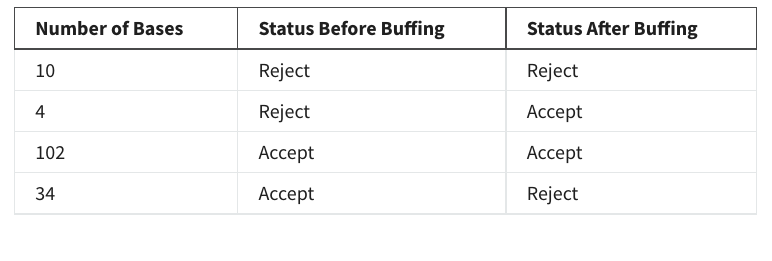
\includegraphics{quiz_36.png}
\caption{Table P36}
\end{figure}

\begin{Shaded}
\begin{Highlighting}[]
\CommentTok{\#Dependency McNemar}
\NormalTok{ct }\OtherTok{=} \FunctionTok{c}\NormalTok{(}\DecValTok{102}\NormalTok{,}\DecValTok{4}\NormalTok{,}\DecValTok{34}\NormalTok{,}\DecValTok{10}\NormalTok{)}
\NormalTok{(ct.new}\OtherTok{\textless{}{-}}\FunctionTok{matrix}\NormalTok{(ct,}\AttributeTok{nrow =} \DecValTok{2}
\NormalTok{                , }\AttributeTok{dimnames =} \FunctionTok{list}\NormalTok{(}\StringTok{"Before Buffing"} \OtherTok{=} \FunctionTok{c}\NormalTok{(}\StringTok{"Accept"}\NormalTok{, }\StringTok{"Reject"}\NormalTok{),}
                                  \StringTok{"After MBuffing"} \OtherTok{=} \FunctionTok{c}\NormalTok{(}\StringTok{"Accept"}\NormalTok{, }\StringTok{"Reject"}\NormalTok{))))}
\end{Highlighting}
\end{Shaded}

\begin{verbatim}
##               After MBuffing
## Before Buffing Accept Reject
##         Accept    102     34
##         Reject      4     10
\end{verbatim}

\begin{Shaded}
\begin{Highlighting}[]
\FunctionTok{mcnemar.test}\NormalTok{(ct.new)}
\end{Highlighting}
\end{Shaded}

\begin{verbatim}
## 
##  McNemar's Chi-squared test with continuity correction
## 
## data:  ct.new
## McNemar's chi-squared = 22.132, df = 1, p-value = 2.546e-06
\end{verbatim}

\hypertarget{section-2}{%
\section{37, 38}\label{section-2}}

\hypertarget{for-38-try-no-way-to-tell}{%
\section{for 38 try no way to tell}\label{for-38-try-no-way-to-tell}}

Question 37 Safety data have been collected in a manufacturing plant for
the past several years. During an initial time period of 2 years, 15
lost-time accidents occurred. A safety improvement program was then
instituted.

During the next 1 year, 10 lost-time accidents occurred. Has the safety
initiative resulted in an improvement in the safety level in the plant
as measured by the lost-time accident rate?.

You may assume the data were tested and conform to a Poisson
distribution. Use a Confidence Level of 95\%.

\begin{Shaded}
\begin{Highlighting}[]
\CommentTok{\#wrong pvalue}
\CommentTok{\#since not rejecting null hypothesis, no way to tell if it made a difference}
\FunctionTok{poisson.test.twosample.simple}\NormalTok{(}\AttributeTok{sample.count.g1 =} \DecValTok{30} \CommentTok{\#we need to use total count so thie case it\textquotesingle{}s 15*30}
\NormalTok{                              ,}\AttributeTok{sample.size.g1 =} \DecValTok{2}
\NormalTok{                              ,}\AttributeTok{sample.count.g2 =} \DecValTok{10}
\NormalTok{                              ,}\AttributeTok{sample.size.g2 =} \DecValTok{1}\NormalTok{)}
\end{Highlighting}
\end{Shaded}

\begin{verbatim}
## 
##  Two-Sample Poisson Test
## 
## data:  sample counts and sample sizes
## z = 1.118, difference in rates = 0, p-value = 0.2636
## alternative hypothesis: true difference in rates is not equal to 0
## 95 percent confidence interval:
##  NA NA
## sample estimates:
##           rate.g1           rate.g2        lambda.hat g1.lambda.lowerci 
##         15.000000         10.000000         13.333333         10.120437 
## g1.lambda.upperci g2.lambda.lowerci g2.lambda.upperci 
##         21.413433          4.795389         18.390356
\end{verbatim}

\end{document}
